Performance engineering of code is achieved in languages that are \textit{close to the machine},\cite{Ritchie} with data types and operations that intuitively and directly correspond to hardware primitives.  A language that abstracts too far away from the hardware may be fast in many cases, but even in these good cases, there are cycles to be gained.  Laying data out differently, possibly by packing some or all of the structure, or forcing a particular alignment, can have significant implications on performance.  Omitting instructructions added by the compiler that guarantee safety, such as bounds-checking, can be a boon when they occur inside a loop.

Consequent, and inextricably linked to this, is the need for tight control over memory allocation.  For this reason, although C and C++ have good, sturdy conservative garbage collectors\cite{BDW}(cite .NET gc), high performance applications tend to avoid it.  Garbage collectors represent a trade-off between performance and code simplicity.  This trade-off makes concurrent data structure implementation difficult in languages that are close to the machine, since most available techniques for concurrent memory reclamation require invasive modification of the operations or place restrictions on how they can be used and where pointers are allowed be stored.\cite{HP}\cite{DTA}\cite{StackTrack}\cite{Threadscan}

High performance benchmarks of concurrent data structures often forgo memory reclamation altogether.\cite{Synchrobench}\cite{Scal}  Literally, they leak the memory or use a cyclical allocator that knows about usage patterns in the benchmark and waits ``long enough'' before reallocating a chunk of memory.  Now, there's a well-reasoned argument to be made for this: Concurrent memory reclamation techniques slow down operations, and we want to know -- in the ideal case -- what is the upper bound on performance for thus-and-such a data structure?  But this upper bound isn't tight because memory reclamation is a real and valid component of performance.  Moreover, inasmuch as the benchmark code lacks memory reclamation, it probably doesn't resemble the production code; no template has been provided that can be drawn upon by application programmers.

The problem of concurrent data structures in languages that are close to the machine is the tension between control over all aspects of performance on individual threads, and the ability to develop the concurrent code in a way that's modular and maintainable.  This is further complicated by the prevalence of legacy code -- applications already written in C or C++ -- that makes selection of a new language impractical.

In this work we introduce DEF, a language designed to integrate seemlessly into C or C++, that provides support for high performance, concurrency programming.  Seemless integration (figure~\ref{fig:seemless-integration}) means that DEF understands C types, data structures, variables, and function declarations and can read them from C header files; and that a C header file can be automatically generated from a DEF source file, allowing C to interface with anything exported from DEF.

\begin{figure}[htbp!]
        \centering
        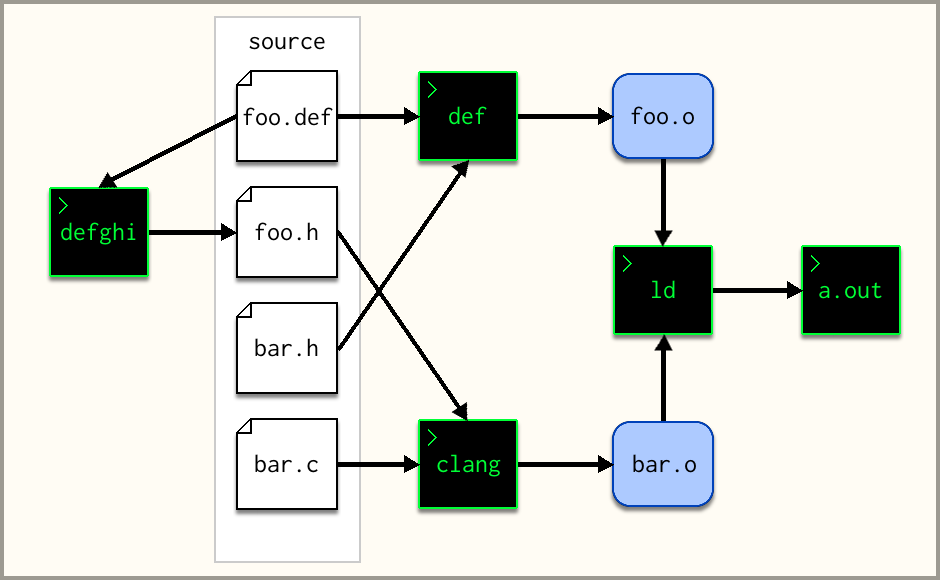
\includegraphics[scale=0.25]{gfx/seemless-integration}
        \caption{Integration between DEF and C source code can be done seemlessly by generating a C header file from the DEF source file, using the \texttt{defghi} utility, and importing/including the necessary header files into the respective source files.  Objects can be linked together as usual.}
        \label{fig:seemless-integration}
\end{figure}

DEF provides primitives for traditional low-level memory management in the form of \texttt{new} and \texttt{delete}, but also adds a \texttt{retire} keyword for use with pointers that may be visible to multiple threads.  The expectation is that memory can be allocated and deallocated, just as it is in normal C programs, and \texttt{new} and \texttt{delete} can be configured to use an application-specific allocator, since performance programmers will look for the one that performs best on their application.  But when memory is shared in a concurrent data structure, \textit{invisible readers}, threads that perform nothing but read operations on a node (and are, therefore, invisible to a thread that might want to free it), memory can be retired and tracked by a special-purpose runtime.  \texttt{retire} is implemented by Forkscan that tracks nothing but retired memory and scales well across many cores.\cite{Forkscan}

By default, DEF's native runtimes are the C runtime library and those that are required for support for concurrency (Forkscan) and parallelism (Cilk\cite{BlumofeCilk}).  Adding DEF to an existing application, therefore, creates no additional burden or potential dependency conflicts.

As proof of concept, we implemented a benchmark suite including various concurrent data structures in DEF with corresponding (leaky) implementations in C. (Brief of results)

